\chapter{Результат}

%На рисунке \ref{fig:ui} представлен консольный интерфейс приложения.
%
%\begin{figure}[H]
%	\centering
%	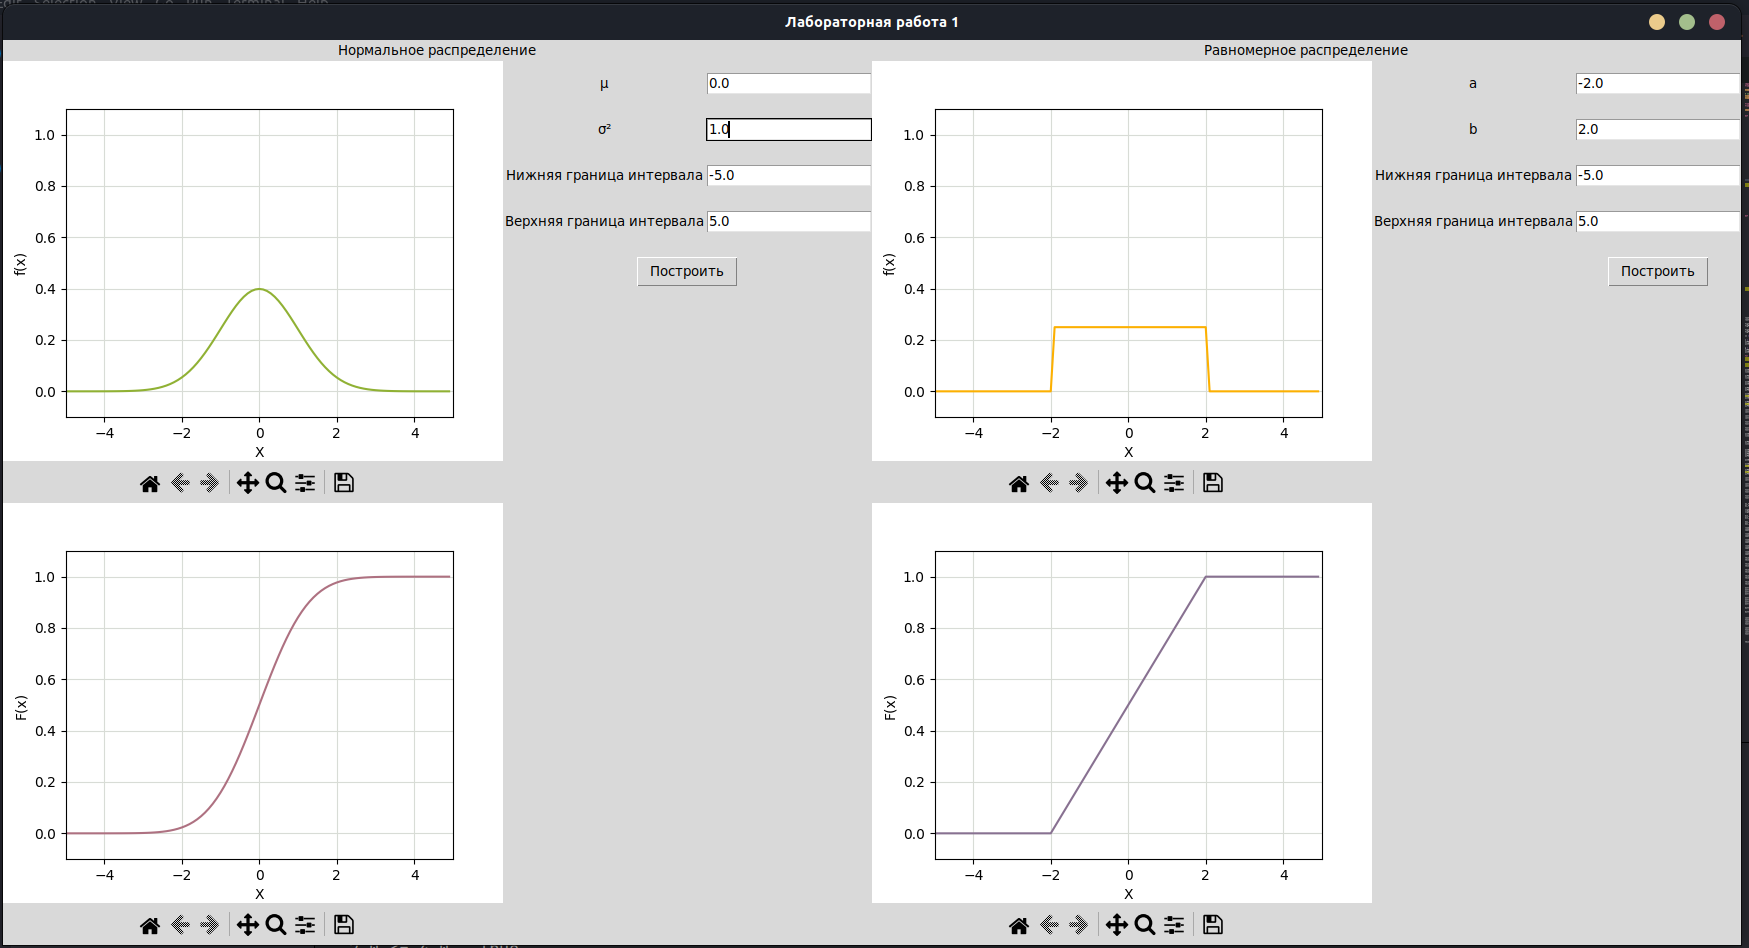
\includegraphics[width=0.7\linewidth]{assets/gui.jpg}
%	\caption{Консольный интерфейс приложения}
%	\label{fig:ui}
%\end{figure}

%\section{Программный интерфейс}
\section{Результаты работы}
На рисунках \ref{fig:r20}, \ref{fig:r40}, \ref{fig:r60} и \ref{fig:r80} приведены результаты работы программы. Параметры: ${N(0 , 0.2), \; U{[1, 10]}}$.

\begin{figure}[H]
	\centering
	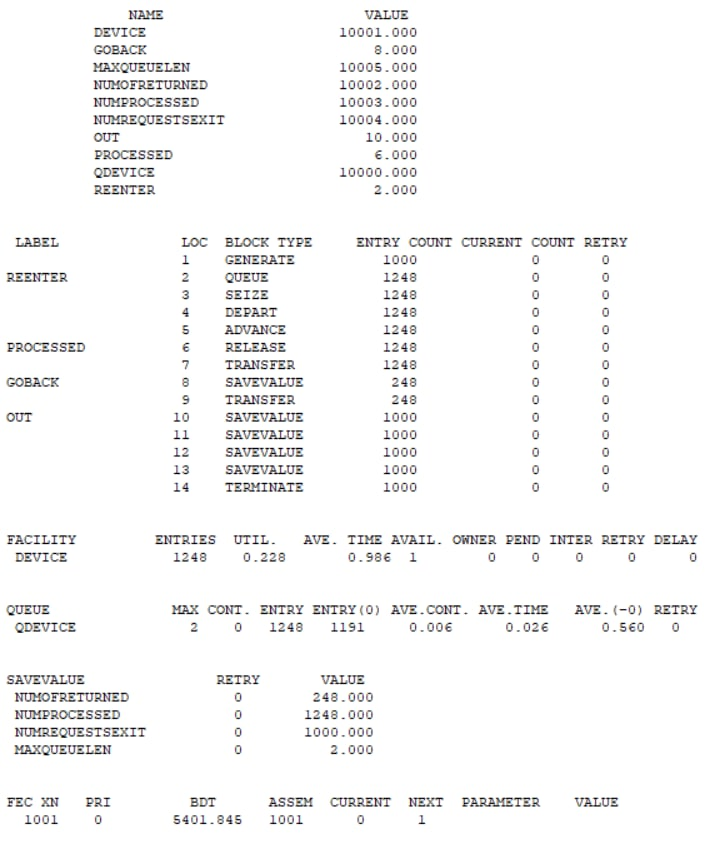
\includegraphics[width=0.85\textwidth]{assets/20.jpg}
	\caption{Результат при обработке 1000 заявок и 20\% повторений}
	\label{fig:r20}
\end{figure}


\begin{figure}[H]
	\centering
	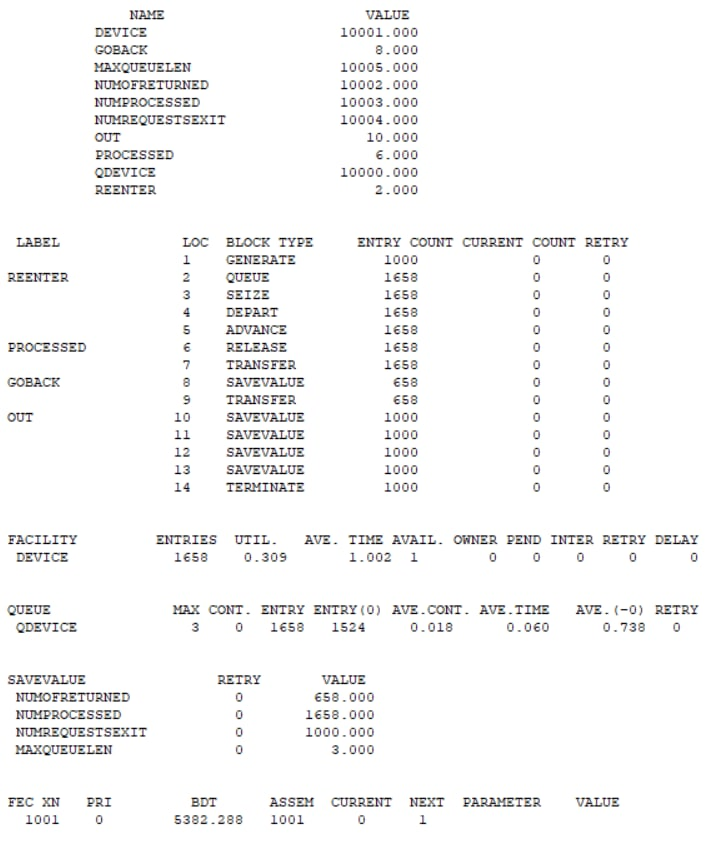
\includegraphics[width=\textwidth]{assets/40.jpg}
	\caption{Результат при обработке 1000 заявок и 40\% повторений}
	\label{fig:r40}
\end{figure}


\begin{figure}[H]
	\centering
	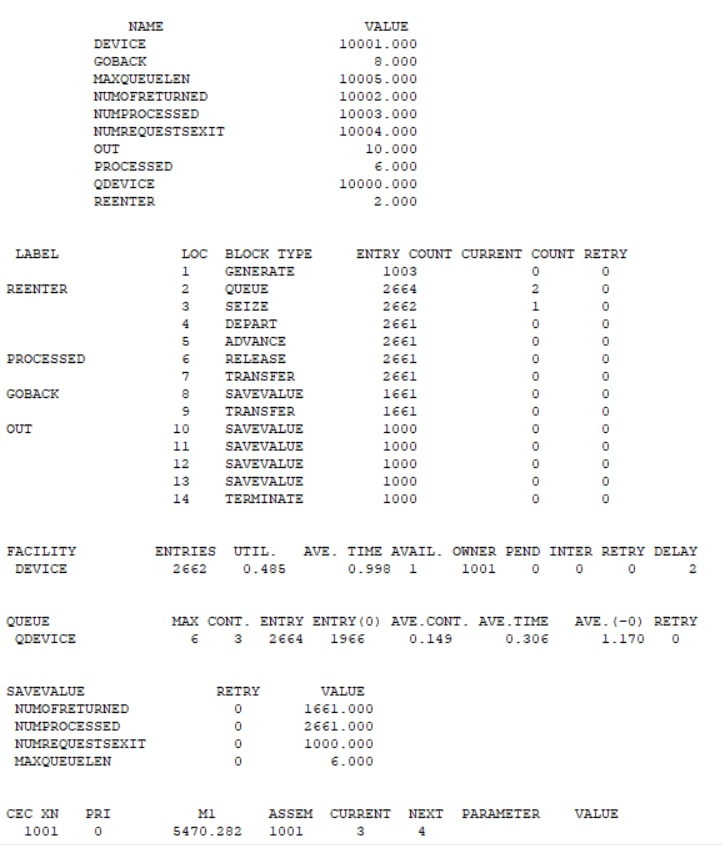
\includegraphics[width=\textwidth]{assets/60.jpg}
	\caption{Результат при обработке 1000 заявок и 60\% повторений}
	\label{fig:r60}
\end{figure}

\begin{figure}[H]
	\centering
	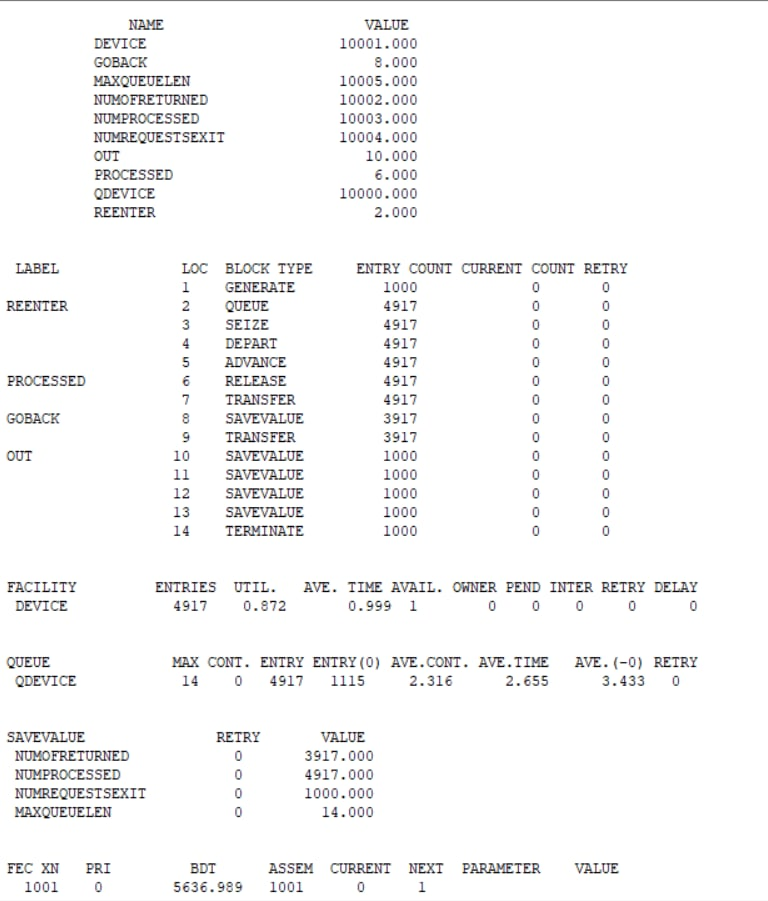
\includegraphics[width=\textwidth]{assets/80.jpg}
	\caption{Результат при обработке 1000 заявок и 80\% повторений}
	\label{fig:r80}
\end{figure}